\begin{frame}{Primo Passo: le entit\`a}
\fboxsep=2pt
\noindent\fbox{%
\begin{minipage}[t]{0.6\linewidth}
\textbf{DATABASE PER A MENSA DELL'ERSU:}
\\ci sono diverse mense a Camerino, situate in diverse zone, in cui si pu\`o mangiare.
\\Ogni mensa cucina diversi tipi di piatti che hanno costi differenti e sono classificati in maniera differente (primo, secondo, etc...)
\\Le mense servono gli studenti universitari e tutte le persone associate all'universit\`a in possesso di un tesserino ERSU.
\\I tesserini possono anche essere provvisori e una persona pu\`o quindi entrare in possesso di pi\`u tesserini.
\\\`E possibile usufruire della mensa 2 volte al giorno.
\end{minipage}}%
\hfill%
\begin{minipage}[t]{0.35\linewidth}
1.~Individuare nel testo tutte le possibili \color{red}{entit\`a}.
\end{minipage}
\end{frame}
%
\begin{frame}{Primo Passo: le entit\`a}
\fboxsep=2pt
\noindent\fbox{%
\begin{minipage}[t]{0.6\linewidth}
\textbf{DATABASE PER A MENSA DELL'ERSU:}
\\ci sono diverse {\color{red}{mense}} a Camerino, situate in diverse zone, in cui si pu\`o mangiare.
\\Ogni mensa cucina diversi tipi di {\color{red}{piatti}} che hanno costi differenti e sono classificati in maniera differente (primo, secondo, etc...)
\\Le mense servono gli {\color{red}{studenti}} universitari e tutte le {\color{red}{persone}} associate all'universit\`a in possesso di un {\color{red}{tesserino}} ERSU.
\\I tesserini possono anche essere provvisori e una persona pu\`o quindi entrare in possesso di pi\`u tesserini.
\\\`E possibile usufruire della mensa 2 volte al giorno.
\end{minipage}}%
\hfill%
\begin{minipage}[t]{0.35\linewidth}
1.~Individuare nel testo tutte le possibili {\color{red}{entit\`a}}.
\pause
\begin{block}{Nota bene}
Quando non \`e chiaro se un oggetto di seconda importanza va considerato o meno come entit\`a basta vedere se ci sono attributi legati ad esso.
\newline
\\esempio: zona o tesserino
\end{block}
\end{minipage}
\end{frame}
%
\begin{frame}{Secondo Passo: gli attributi}
\fboxsep=2pt
\noindent\fbox{%
\begin{minipage}[t]{0.6\linewidth}
\textbf{DATABASE PER A MENSA DELL'ERSU:}
\\ci sono diverse {\color{red}{mense}} a Camerino, situate in diverse zone, in cui si pu\`o mangiare.
\\Ogni mensa cucina diversi tipi di {\color{red}{piatti}} che hanno costi differenti e sono classificati in maniera differente (primo, secondo, etc...)
\\Le mense servono gli {\color{red}{studenti}} universitari e tutte le {\color{red}{persone}} associate all'universit\`a in possesso di un {\color{red}{tesserino}} ERSU.
\\I tesserini possono anche essere provvisori e una persona pu\`o quindi entrare in possesso di pi\`u tesserini.
\\\`E possibile usufruire della mensa 2 volte al giorno.
\end{minipage}}%
\hfill%
\begin{minipage}[t]{0.35\linewidth}
2.~Individuare nel testo tutti i possibili \color{blue}{attributi}.
\end{minipage}
\end{frame}
%
\begin{frame}{Secondo Passo: gli attributi}
\fboxsep=2pt
\noindent\fbox{%
\begin{minipage}[t]{0.6\linewidth}
\textbf{DATABASE PER A MENSA DELL'ERSU:}
\\ci sono diverse {\color{red}{mense}} a Camerino, situate in diverse {\color{blue}{zone}}, in cui si pu\`o mangiare.
\\Ogni mensa cucina diversi tipi di {\color{red}{piatti}} che hanno {\color{blue}{costi}} differenti e sono {\color{blue}{classificati}} in maniera differente (primo, secondo, etc...)
\\Le mense servono gli {\color{red}{studenti}} universitari e tutte le {\color{red}{persone}} associate all'universit\`a in possesso di un {\color{red}{tesserino}} ERSU.
\\I tesserini possono anche essere {\color{blue}{provvisori}} e una persona pu\`o quindi entrare in possesso di pi\`u tesserini.
\\\`E possibile usufruire della mensa 2 volte al {\color{blue}{giorno}}.
\end{minipage}}%
\hfill%
\begin{minipage}[t]{0.35\linewidth}
\vspace{.3cm}
2.~Individuare nel testo tutti i possibili {\color{blue}{attributi}}.
\pause
\begin{block}{Nota bene}
A volte nei testi alcuni attributi non vengono specificati perch\'e \`e scontato che sono necessari.
\vspace{.3cm}
esempio: i nomi delle persone.
\pause
\vspace{.3cm}

Bisogna comunque tenere sempre a mente che aggiungere attributi inutili e non richiesti non \`e mai una buona pratica.
\end{block}
\end{minipage}
\end{frame}
%
\begin{frame}{Terzo Passo: Bozza ER}
\fboxsep=2pt
\noindent\fbox{%
\begin{minipage}[t]{0.6\linewidth}
\textbf{DATABASE PER A MENSA DELL'ERSU:}
\\ci sono diverse {\color{red}{mense}} a Camerino, situate in diverse {\color{blue}{zone}}, in cui si pu\`o mangiare.
\\Ogni mensa cucina diversi tipi di {\color{red}{piatti}} che hanno {\color{blue}{costi}} differenti e sono {\color{blue}{classificati}} in maniera differente (primo, secondo, etc...)
\\Le mense servono gli {\color{red}{studenti}} universitari e tutte le {\color{red}{persone}} associate all'universit\`a in possesso di un {\color{red}{tesserino}} ERSU.
\\I tesserini possono anche essere {\color{blue}{provvisori}} e una persona pu\`o quindi entrare in possesso di pi\`u tesserini.
\\\`E possibile usufruire della mensa 2 volte al {\color{blue}{giorno}}.
\end{minipage}}%
\hfill%
\begin{minipage}[t]{0.35\linewidth}
\vspace{.3cm}
3.~Iniziare una bozza del diagramma con le entit\`a e gli attributi presi in considerazione.
\pause
\begin{block}{\small Nota bene}
{\small Se in una consegna complessa non si riesce a capire a chi appartenga un determinato attributo conviene ragionarci in seguito.}
\pause
\vspace{.3cm}

{\small Potrebbe capitare che l'attributo \`e di un'associazione, quindi basta segnarselo e lavorarci in un secondo momento. (es. giorno)}
\end{block}
\end{minipage}
\end{frame}
%
\begin{frame}{Terzo Passo: Bozza ER}
\begin{minipage}[t]{0.6\linewidth}
\begin{figure}
    \centering
    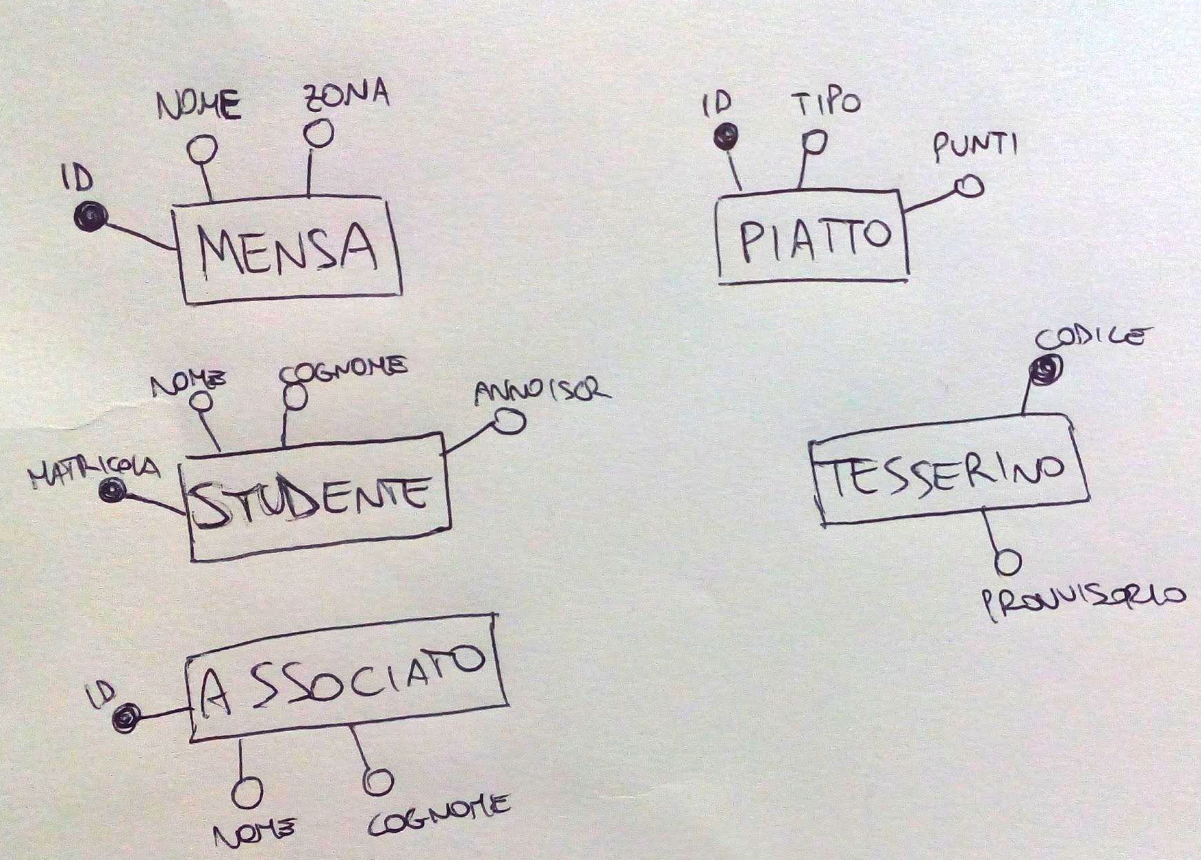
\includegraphics[width=\textwidth]{img/bozza-er.png}
\end{figure}
\end{minipage}%
\hfill%
\begin{minipage}[t]{0.35\linewidth}
\vspace{.3cm}
\begin{itemize}[<+->]
    \item Si inizia sempre scrivendo tutte le entit\`a e gli attributi;
    \item I pi\`u pigri tendono a scrivere gli attributi alla fine, conviene invece scriverli subito in modo da riconoscere facilmente le generalizzazioni IS-A e modellare correttamente le associazioni.
\end{itemize}
\end{minipage}
\end{frame}
%
\begin{frame}{Terzo Passo: Bozza ER}
\vspace{-.65cm}
\begin{figure}
    \centering
    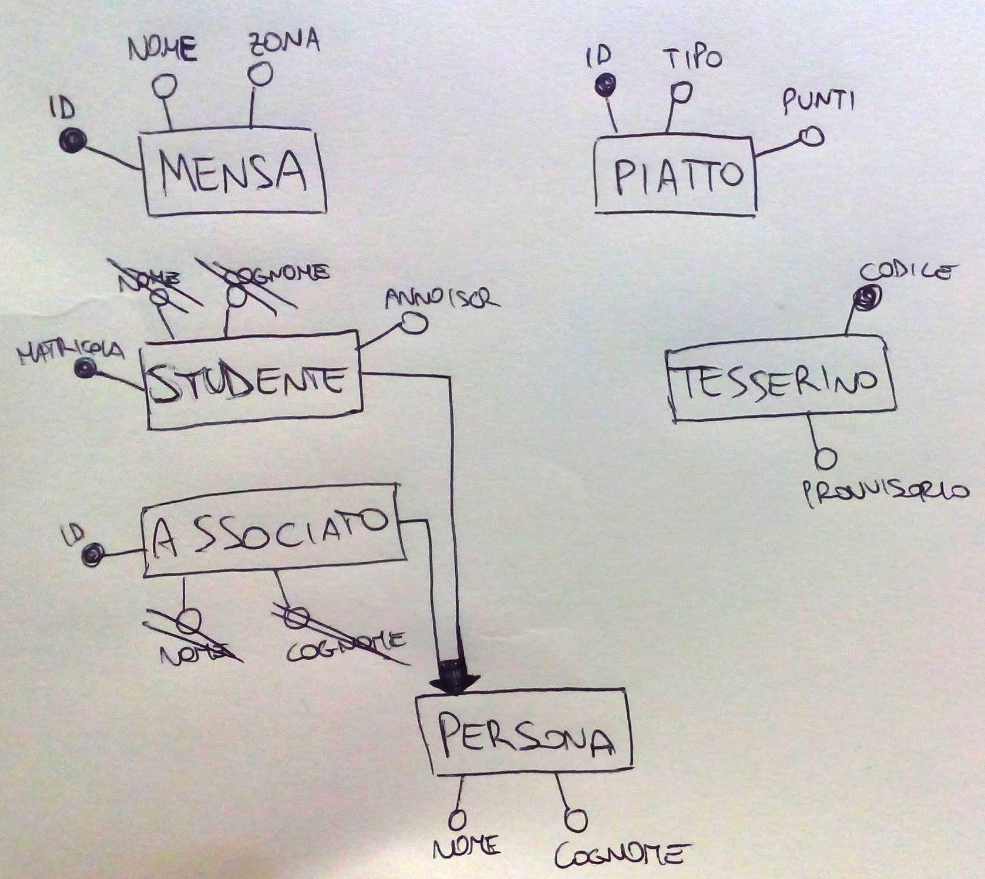
\includegraphics[width=.55\textwidth]{img/bozza-er-generalizzazioni.png}
\end{figure}
\end{frame}
%
\begin{frame}{Quarto Passo: Associazioni}
\fboxsep=2pt
\noindent\fbox{%
\begin{minipage}[t]{0.6\linewidth}
\textbf{DATABASE PER A MENSA DELL'ERSU:}
\\ci sono diverse {\color{red}{mense}} a Camerino, situate in diverse {\color{blue}{zone}}, in cui si pu\`o mangiare.
\\Ogni mensa cucina diversi tipi di {\color{red}{piatti}} che hanno {\color{blue}{costi}} differenti e sono {\color{blue}{classificati}} in maniera differente (primo, secondo, etc...)
\\Le mense servono gli {\color{red}{studenti}} universitari e tutte le {\color{red}{persone}} associate all'universit\`a in possesso di un {\color{red}{tesserino}} ERSU.
\\I tesserini possono anche essere {\color{blue}{provvisori}} e una persona pu\`o quindi entrare in possesso di pi\`u tesserini.
\\\`E possibile usufruire della mensa 2 volte al {\color{blue}{giorno}}.
\end{minipage}}%
\hfill%
\begin{minipage}[t]{0.35\linewidth}
\vspace{.1cm}
4.~Collegare le entit\`a con le dovute {\color{magenta}{associazioni}} specificandone le cardinalit\`a.
\vspace{-.1cm}
\pause
\begin{block}{\small Nota bene}
{\small Spesso le associazioni (e le cardinalit\`a) sono dettate dal buon senso, quindi non vengono specificate nel testo.}
\pause
\vspace{.3cm}

{\small Tuttavia, per casi particolari, vengono richieste delle associazioni in maniera esplicita, vanno quindi scovate nel testo per una corretta modellazione.}
\end{block}
\end{minipage}
\end{frame}
%
\begin{frame}{Quarto Passo: Associazioni}
\fboxsep=2pt
\noindent\fbox{%
\begin{minipage}[t]{0.6\linewidth}
\textbf{DATABASE PER A MENSA DELL'ERSU:}
\\ci sono diverse {\color{red}{mense}} a Camerino, situate in diverse {\color{blue}{zone}}, in cui si pu\`o mangiare.
\\Ogni mensa cucina diversi tipi di {\color{red}{piatti}} che hanno {\color{blue}{costi}} differenti e sono {\color{blue}{classificati}} in maniera differente (primo, secondo, etc...)
\\Le mense servono gli {\color{red}{studenti}} universitari e tutte le {\color{red}{persone}} associate all'universit\`a in possesso di un {\color{red}{tesserino}} ERSU.
\\I tesserini possono anche essere {\color{blue}{provvisori}} e una persona pu\`o quindi entrare in {\color{magenta}{possesso}} di pi\`u tesserini.
\\\`E possibile usufruire della mensa 2 volte al {\color{blue}{giorno}}.
\end{minipage}}%
\hfill%
\begin{minipage}[t]{0.35\linewidth}
\vspace{.1cm}
4.~Collegare le entit\`a con le dovute {\color{magenta}{associazioni}} specificandone le cardinalit\`a.
\vspace{-.1cm}
\begin{block}{\small Nota bene}
{\small Spesso le associazioni (e le cardinalit\`a) sono dettate dal buon senso, quindi non vengono specificate nel testo.}
\vspace{.3cm}

{\small Tuttavia, per casi particolari, vengono richieste delle associazioni in maniera esplicita, vanno quindi scovate nel testo per una corretta modellazione.}
\end{block}
\end{minipage}
\end{frame}
%
\begin{frame}{Quarto Passo: Nomi associazioni}
\begin{minipage}[t]{0.6\linewidth}
\vspace{-1cm}
    \begin{figure}
        \centering
        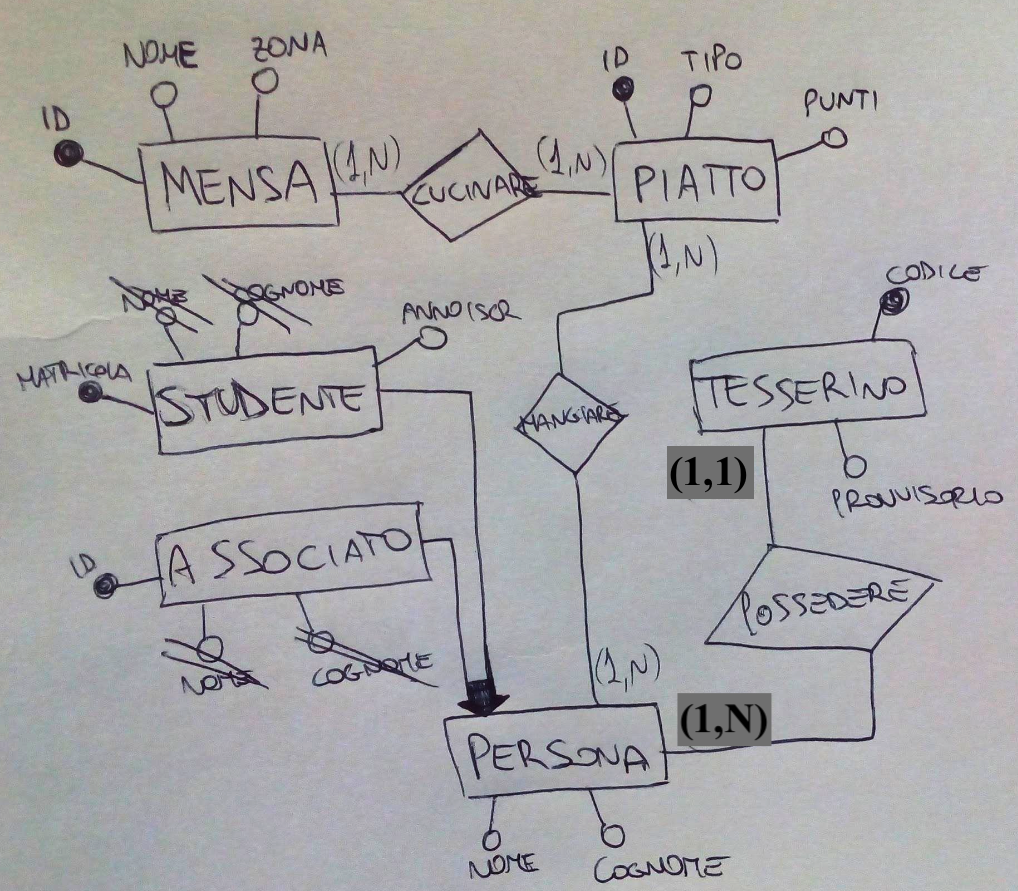
\includegraphics[width=.9\textwidth]{img/er-dopo-quarto-passo.png}
    \end{figure}
\end{minipage}%
\hfill%
\begin{minipage}[t]{0.35\linewidth}
\vspace{.3cm}
\begin{itemize}[<+->]
    \item A volte trovare i nomi per le associazioni pu\`o risultare arduo. In questi casi conviene ignorare il nome e proseguire con il progetto, per i nomi c'\`e tempo.
\end{itemize}
\end{minipage}
\end{frame}
%
\begin{frame}{Quinto Passo: Rileggere e controllare}
\fboxsep=2pt
\noindent\fbox{%
\begin{minipage}[t]{0.6\linewidth}
\textbf{DATABASE PER A MENSA DELL'ERSU:}
\\ci sono diverse {\color{red}{mense}} a Camerino, situate in diverse {\color{blue}{zone}}, in cui si pu\`o mangiare.
\\Ogni mensa cucina diversi tipi di {\color{red}{piatti}} che hanno {\color{blue}{costi}} differenti e sono {\color{blue}{classificati}} in maniera differente (primo, secondo, etc...)
\\Le mense servono gli {\color{red}{studenti}} universitari e tutte le {\color{red}{persone}} associate all'universit\`a in possesso di un {\color{red}{tesserino}} ERSU.
\\I tesserini possono anche essere {\color{blue}{provvisori}} e una persona pu\`o quindi entrare in {\color{magenta}{possesso}} di pi\`u tesserini.
\\\`E possibile usufruire della mensa 2 volte al {\color{blue}{giorno}}.
\end{minipage}}%
\hfill%
\begin{minipage}[t]{0.35\linewidth}
\vspace{.1cm}
5.~Rileggere passo passo il testo e controllare che il diagramma soddisfi tutte le richieste.
\vspace{-.1cm}
\pause
\begin{block}{\small Nota bene}
{\small Se ci sono degli elementi lasciati in sospeso bisogna inserirli nel modello!}
\end{block}
\end{minipage}
\end{frame}
%
\begin{frame}{Quinto Passo: Rileggere e controllare}
\begin{minipage}[t]{0.6\linewidth}
\vspace{-1cm}
    \begin{figure}
        \centering
        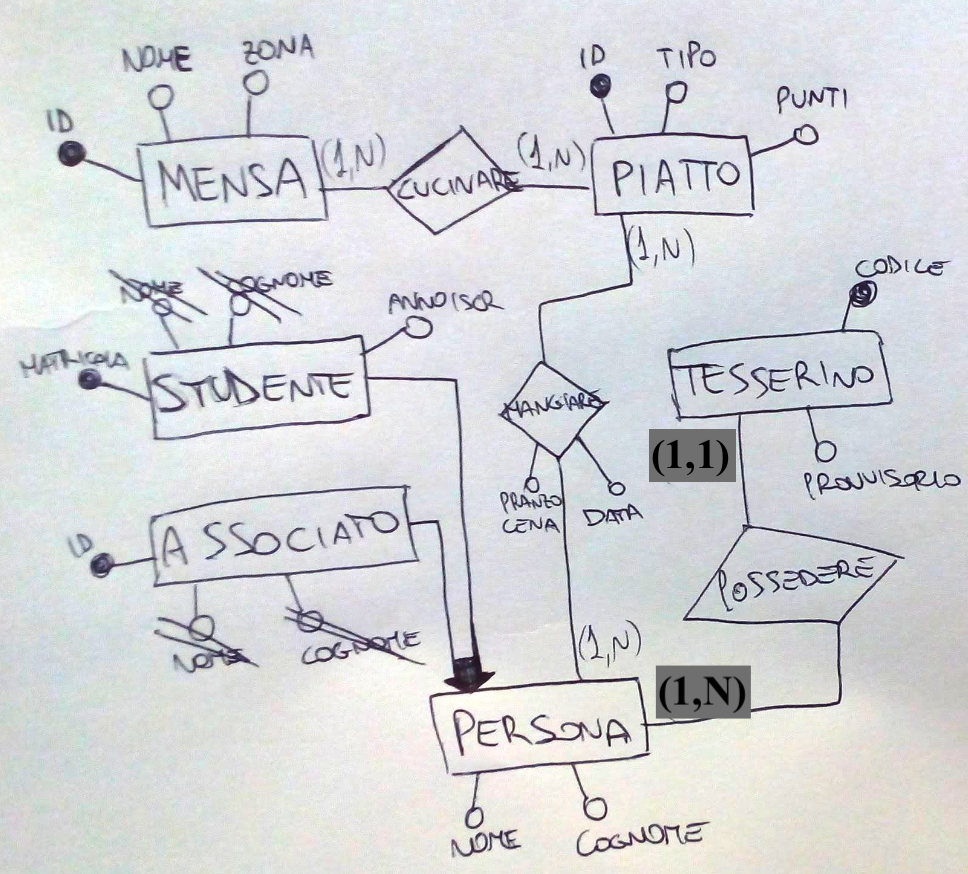
\includegraphics[width=.9\textwidth]{img/er-dopo-quinto-passo.png}
    \end{figure}
\end{minipage}%
\hfill%
\begin{minipage}[t]{0.35\linewidth}
\vspace{.3cm}
\begin{itemize}[<+->]
    \item In questo tipo di esercizi \textbf{non esiste UNA soluzione}, ma ce ne possono essere diverse!
\end{itemize}
\end{minipage}
\end{frame}
%